\section{Backup Slides}

\begin{frame}{Problems of LLMs}
    \begin{columns}[T]
        \begin{column}{0.70\textwidth}
            The works aimed at correcting LLMs can be classified according to the issues they tackle:
            \begin{enumerate}
                \item Hallucination: plausible-sounding but false information~\cite{gao2023rarr, zhang2023language}.

                \item Unfaithful Reasoning: derived conclusion does not follow the previously generated reasoning chain~\cite{he2022rethinking, pan2023logiclm}.

                \item Toxic Contents: content that is toxic, biased, or harmful due to biases present in the training datas~\cite{lu2022quark, gou2023critic}.

                \item Flawed Codes: flawed or incorrect code generation~\cite{chen2023teaching, olausson2023selfrepair}.
            \end{enumerate}
        \end{column}
        \begin{column}{0.30\textwidth}
            \begin{figure}[!htb]
                \centering
                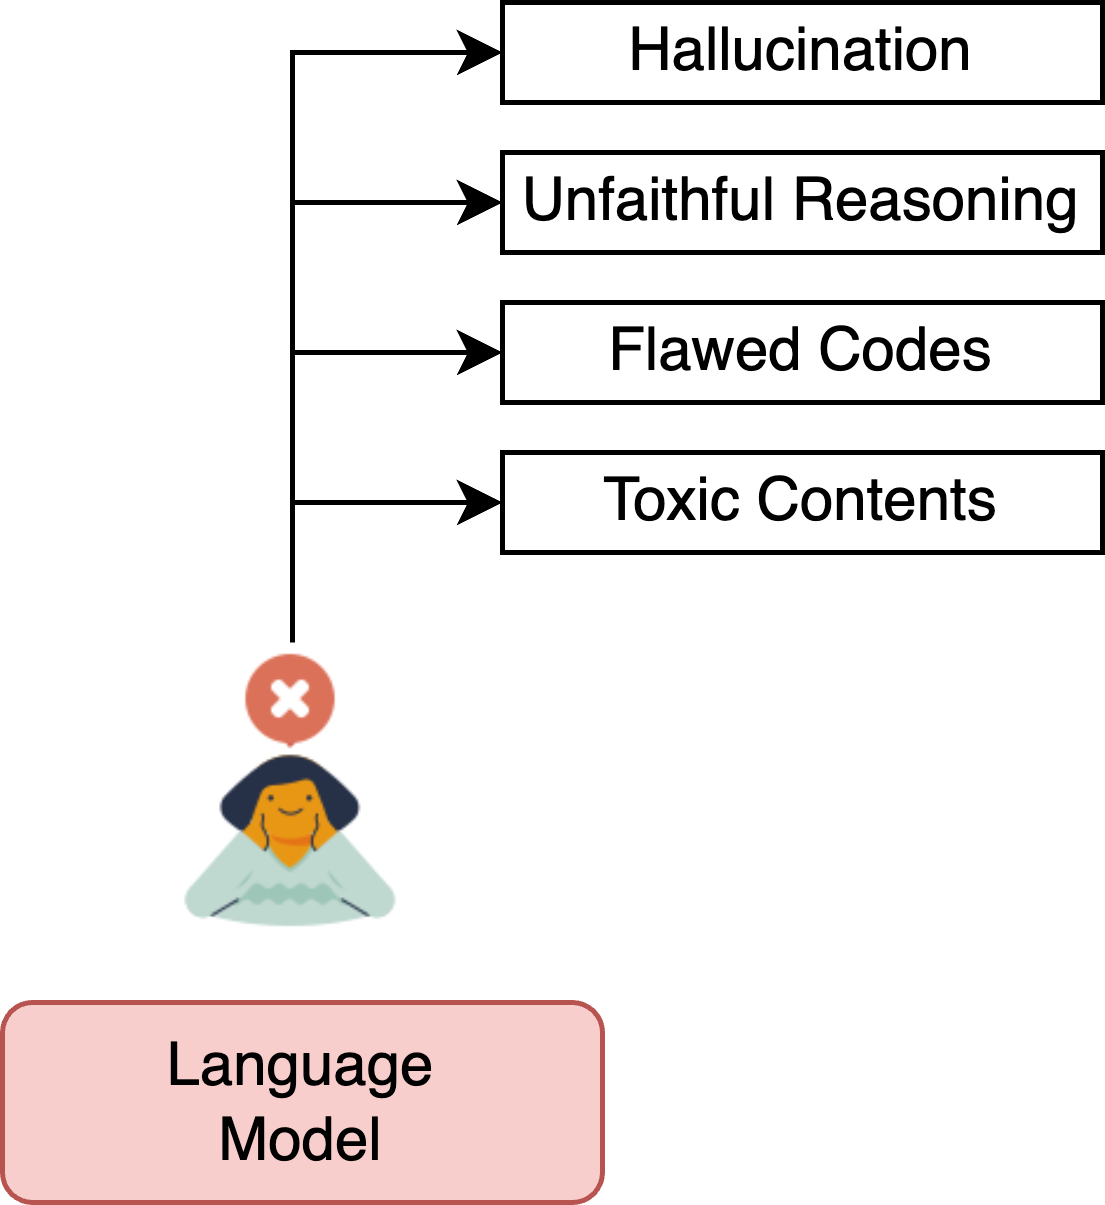
\includegraphics[width=1\textwidth]{img/language_model}
                \captionsetup{font=small,labelformat=empty}
                \caption{Problems of LLMs.}
            \end{figure}
        \end{column}
    \end{columns}
\end{frame}

\begin{frame}{Critic Model}
    \begin{columns}[T]
        \begin{column}{0.55\textwidth}
            Source of feedback:
            \begin{enumerate}
                \item Self-Feedback: the model itself generates feedback~\cite{weng2023large}.

                \item External Feedback: the model receives feedback from an external source (e.g., human, program executor and external knowledge)~\cite{gou2023critic}.
            \end{enumerate}

            Format of feedback:
            \begin{enumerate}
                \item Scalar Value: metrics based on pre-defined tests~\cite{weng2023large}.

                \item Natural Language: provides richer information than scalar value feedback~\cite{chen2023teaching}.
            \end{enumerate}
        \end{column}
        \begin{column}{0.45\textwidth}
            \begin{figure}[!htb]
                \centering
                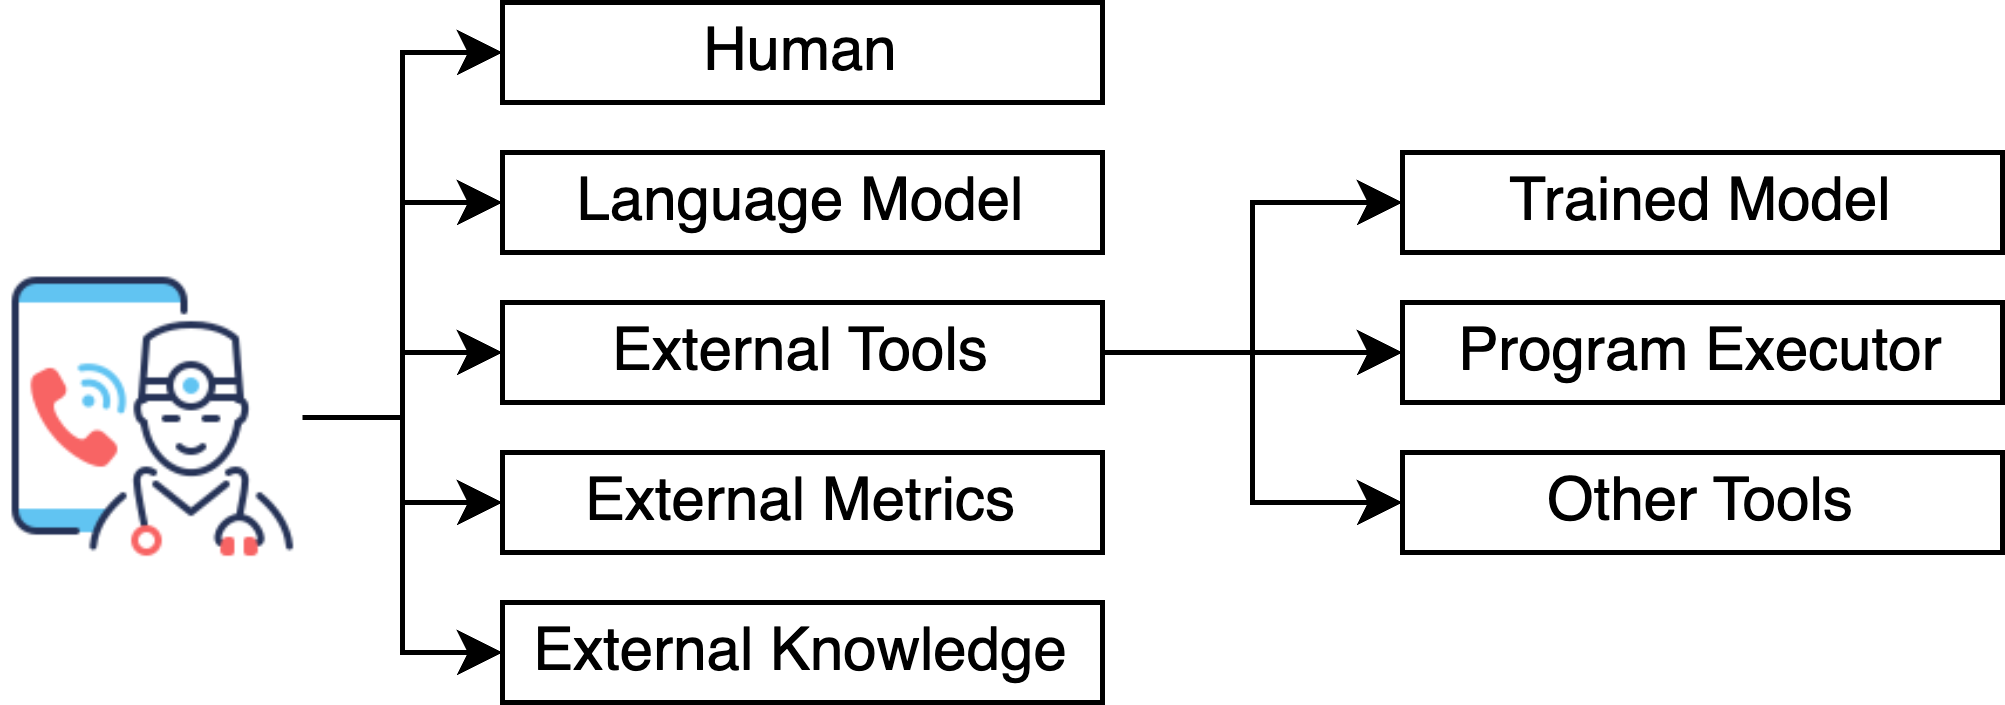
\includegraphics[width=1\textwidth]{img/critic_model}
                \captionsetup{font=small,labelformat=empty}
                \caption{Critic Model.}
            \end{figure}
        \end{column}
    \end{columns}
\end{frame}
